\documentclass[border=6pt]{standalone}
% Shared draw.io-matching colours and node styles for the thesis flowcharts.
\usepackage{tikz}
\usetikzlibrary{shapes.geometric, arrows.meta, positioning, calc}

% Keep words whole inside boxes (no ugly mid-word hyphenation)
\hyphenpenalty=10000\exhyphenpenalty=10000\tolerance=2000

% draw.io standard palette (fill + stroke)
\definecolor{dioBlueF}{HTML}{DAE8FC}\definecolor{dioBlueS}{HTML}{6C8EBF}
\definecolor{dioOrangeF}{HTML}{FFE6CC}\definecolor{dioOrangeS}{HTML}{D79B00}
\definecolor{dioGrayF}{HTML}{F5F5F5}\definecolor{dioGrayS}{HTML}{666666}
\definecolor{dioGreenF}{HTML}{D5E8D4}\definecolor{dioGreenS}{HTML}{82B366}
\definecolor{dioPurpleF}{HTML}{E1D5E7}\definecolor{dioPurpleS}{HTML}{9673A6}

\tikzset{
  >={Stealth[length=2.4mm]},
  fnode/.style={rounded corners=5pt, draw, line width=0.8pt,
    minimum width=2.7cm, minimum height=1.15cm, align=center,
    font=\small, text width=2.5cm, inner sep=2pt},
  blue/.style ={fnode, fill=dioBlueF,   draw=dioBlueS},
  orange/.style={fnode, fill=dioOrangeF, draw=dioOrangeS},
  gray/.style ={fnode, fill=dioGrayF,   draw=dioGrayS},
  green/.style={fnode, fill=dioGreenF,  draw=dioGreenS},
  purple/.style={fnode, fill=dioPurpleF, draw=dioPurpleS},
  decision/.style={diamond, draw, line width=0.8pt, aspect=1.7,
    align=center, font=\small, text width=1.9cm, inner sep=0pt,
    fill=dioGrayF, draw=dioGrayS, minimum width=3cm, minimum height=2.3cm},
  bdecision/.style={decision, fill=dioBlueF, draw=dioBlueS},
  flow/.style={->, line width=0.8pt, draw=black!75},
  elabel/.style={font=\footnotesize, inner sep=1.5pt, fill=white},
}

\begin{document}
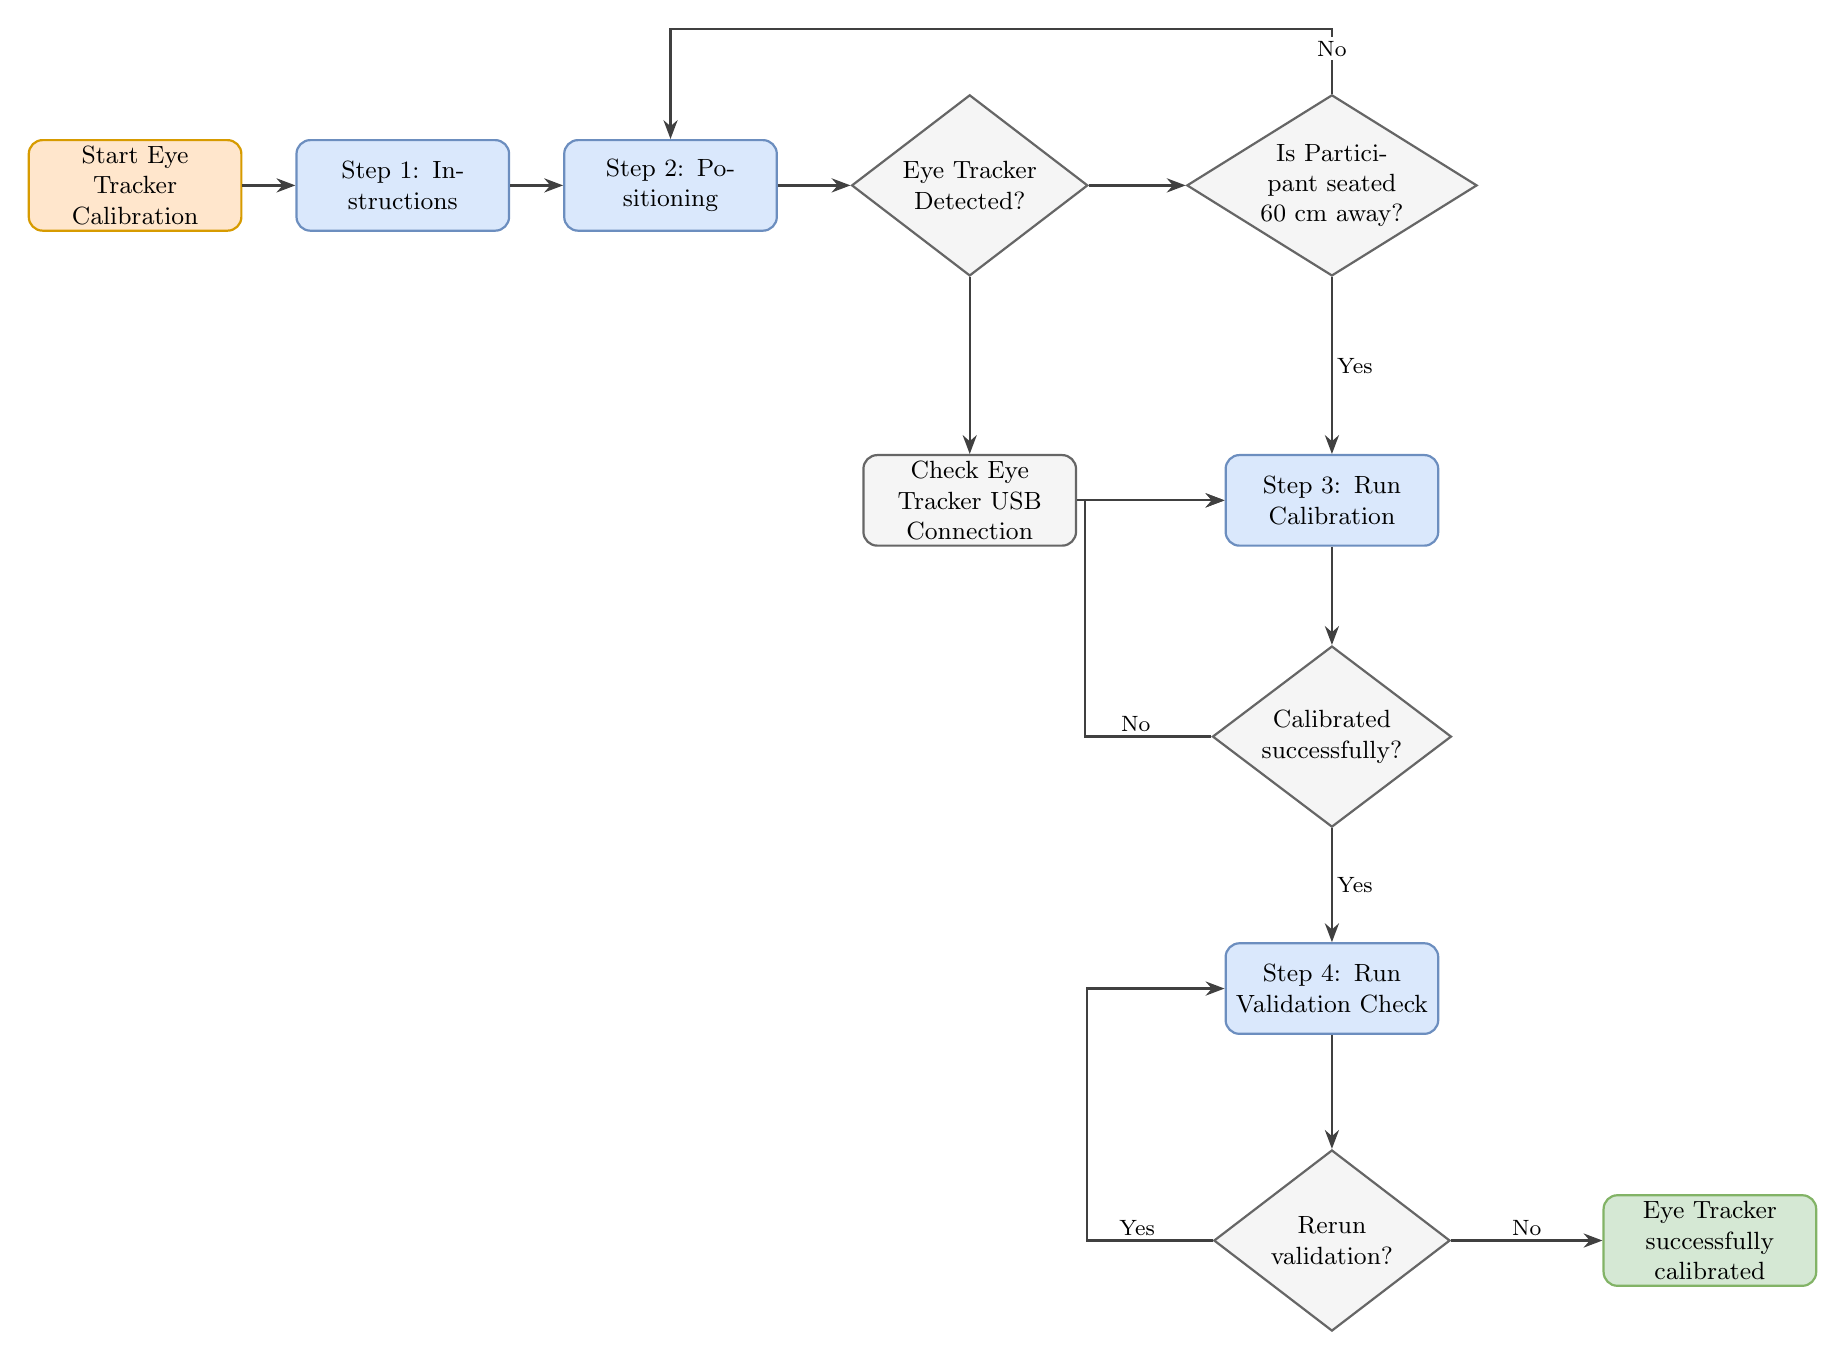
\begin{tikzpicture}[node distance=0pt]

  % ---- Nodes -------------------------------------------------------------
  \node[orange] (start) at (0,0)      {Start Eye Tracker Calibration};
  \node[blue]   (step1) at (3.4,0)    {Step 1: Instructions};
  \node[blue]   (step2) at (6.8,0)    {Step 2: Positioning};
  \node[decision](det)  at (10.6,0)   {Eye Tracker Detected?};
  \node[decision](seat) at (15.2,0)   {Is Participant seated 60 cm away?};

  \node[gray]   (usb)   at (10.6,-4)  {Check Eye Tracker USB Connection};
  \node[blue]   (step3) at (15.2,-4)  {Step 3: Run Calibration};

  \node[decision](calok)at (15.2,-7)  {Calibrated successfully?};
  \node[blue]   (step4) at (15.2,-10.2){Step 4: Run Validation Check};
  \node[decision](rerun)at (15.2,-13.4){Rerun validation?};
  \node[green]  (done)  at (20,-13.4) {Eye Tracker successfully calibrated};

  % ---- Edges -------------------------------------------------------------
  \draw[flow] (start) -- (step1);
  \draw[flow] (step1) -- (step2);
  \draw[flow] (step2) -- (det);
  \draw[flow] (det)   -- (seat);
  \draw[flow] (det)   -- (usb);
  \draw[flow] (usb)   -- (step3);

  % seated? Yes -> run calibration ; No -> back up to positioning
  \draw[flow] (seat) -- node[elabel,right]{Yes} (step3);
  \draw[flow] (seat.north) |- ($(step2.north)+(0,1.4)$)
        node[elabel,pos=0.25,above]{No} -- (step2.north);

  % run calibration -> calibrated? ; No loops back, Yes -> validation
  \draw[flow] (step3) -- (calok);
  \draw[flow] (calok.west) -- ++(-1.6,0) node[elabel,pos=0.6,above]{No} |- (step3.west);
  \draw[flow] (calok) -- node[elabel,right]{Yes} (step4);

  % validation -> rerun? ; Yes loops back, No -> done
  \draw[flow] (step4) -- (rerun);
  \draw[flow] (rerun.west) -- ++(-1.6,0) node[elabel,pos=0.6,above]{Yes} |- (step4.west);
  \draw[flow] (rerun) -- node[elabel,above]{No} (done);

\end{tikzpicture}
\end{document}
